\documentclass{article}

% Chinese Support using xeCJK
% \usepackage{xeCJK}
% \setCJKmainfont{SimSun}

% Chinese Support using CTeX
\usepackage{ctex}

% Math Support
\usepackage{amsmath}
\usepackage{amsfonts}
\usepackage{amssymb}
\usepackage{wasysym}
\newcommand{\angstrom}{\text{\normalfont\AA}}

% Graphics Support
\usepackage{graphicx}
\usepackage{float}

% Reduced page margin
\usepackage{geometry}
\geometry{a4paper,scale=0.8}

\usepackage{caption}
\usepackage{subcaption}

% d and e should be math operators
\newcommand*{\dif}{\mathop{}\!\mathrm{d}}
\newcommand*{\md}{\mathop{}\!\mathrm{d}}
\newcommand*{\me}{\mathrm{e}}

% No indent for each paragraph
% \usepackage{parskip}
% \setlength{\parindent}{0cm}

% Bold style for Greek letters
\usepackage{bm}
\let\Oldmathbf\mathbf
\renewcommand{\mathbf}[1]{\boldsymbol{\Oldmathbf{#1}}}

% More space for dfrac in cell
\usepackage{cellspace}
\setlength{\cellspacetoplimit}{5pt}
\setlength{\cellspacebottomlimit}{5pt}

% SI units
\newcommand{\si}[1]{\  \mathrm{#1}}

% Multi-line author information
\usepackage{authblk}
\author{物理(4+4)1801 \quad  胡喜平 \quad U201811966}
\affil{个人网站 https://hxp.plus/ \quad 电子邮件 hxp201406@gmail.com}

\title{近代物理实验预习笔记——材料形貌及光学性质表征}

\begin{document}

\maketitle

\section{实验目的}

\begin{itemize}
  
\item 学会使用原子力显微镜,并掌握其工作原理。
  
\item 了解材料特性如结构、形貌、组分、光学的表征方法。
  
\item 熟悉紫外分光光度计的工作原理、样品投射(吸收)光谱的测量方法以及禁带宽度的计算。

\end{itemize}

\section{实验内容}

\begin{itemize}
\item 调节原子力显微镜,改变扫描模式,观测不同样品的表面样貌。
\item 通过使用紫外分光光度计测量不同宽度的$ZnO$或者$TiO_2$薄膜的透射光谱,计算样品的光学禁带宽度。
\end{itemize}

\section{实验原理}

\subsection{原子力显微镜(AFM)的原理}

如图(a)所示,微悬臂上的探针距离待测表面很近,待测表面的原子和探针上的原子之间有引力或者斥力,使得微悬臂微小形变。激光打在微悬臂上反射,使得微悬臂的微小变化造成反射激光角度变化,进而测量探针和原子之间的距离。

\begin{figure}[H]
  \centering
  \begin{subfigure}{.25\textwidth}
    \centering
    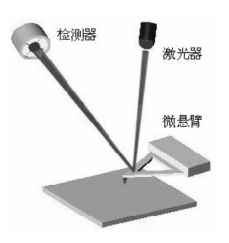
\includegraphics[width=\linewidth]{figures/AFM}
    \caption{AFM测量原理示意简图}
  \end{subfigure}
  \begin{subfigure}{.35\textwidth}
    \centering
    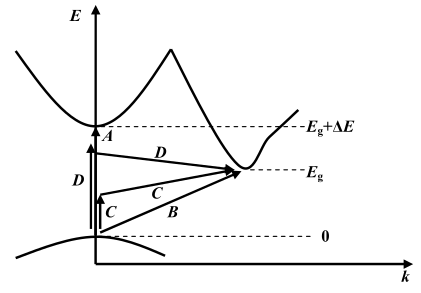
\includegraphics[width=\linewidth]{figures/禁戒的代间直接跃迁}
    \caption{价电子的代间跃迁}
  \end{subfigure}
    \begin{subfigure}{.35\textwidth}
    \centering
    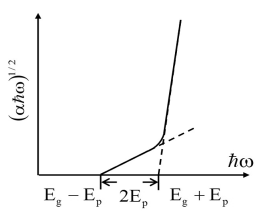
\includegraphics[width=\linewidth]{figures/间接跃迁情况下吸收系数}
    \caption{价电子间接跃迁光学禁带宽度的计算}
  \end{subfigure}
\end{figure}

\subsection{带隙之间直接跃迁和间接跃迁}

图(b)中,入射光子能量大于$E_g + \Delta E$时,发生像箭头A那样的直接跃迁。能量介于$E_g$到$E_g + \Delta E$之间时,发生像箭头B那样的间接跃迁。

其中间接跃迁大致分为两种情况,C过程是吸收声子的,D过程是放出声子的。声子的能量是$E_p$,则C过程光子能量$E_g - E_p$,D过程光子能量$E_g + E_p$。

对于间接跃迁,光子的吸收系数$\alpha$与入射光子能量有平方关系,因此我们做图(c)可以求出光学禁带宽度$E_g$。

实验中能从仪器上获得的数据是透射率$T$,应当用$T$计算吸光度$A$,即

\begin{equation*}
  \begin{aligned}
    A = \lg \dfrac{1}{T} 
  \end{aligned}
\end{equation*}

之后运用朗伯-比尔定律,即$A$正比与$\alpha$。
 
\end{document} 
